\documentclass[a4paper,10pt]{article}
\usepackage{graphicx}
\usepackage{enumitem}
\usepackage{amsmath}
\usepackage{listings}
\usepackage[usenames,dvipsnames]{color}
\usepackage{bbm}
\usepackage{amsfonts}


%%%%%%%%%%%%%%%%%%%%%%%%%%%%%%%%%%%%%%%%%%%%%%%%%%%%%%%%%%%%%%%%%%%%%%%%%%%%%%%%%%%%%%%%%%%
% MATLAB code listing
%
% This is the color used for MATLAB comments below
\definecolor{MyDarkGreen}{rgb}{0.0,0.4,0.0}
 
% For faster processing, load Matlab syntax for listings
\lstloadlanguages{Matlab}%
\lstset{language=Matlab, % Use MATLAB
frame=single, % Single frame around code
basicstyle=\tiny\ttfamily, % Use small true type font
keywordstyle=[1]\color{Blue}\bfseries, % MATLAB functions bold and blue
keywordstyle=[2]\color{Purple}, % MATLAB function arguments purple
keywordstyle=[3]\color{Blue}\underbar, % User functions underlined and blue
identifierstyle=, % Nothing special about identifiers
% Comments small dark green courier
commentstyle=\usefont{T1}{pcr}{m}{sl}\color{MyDarkGreen}\small,
stringstyle=\color{Purple}, % Strings are purple
showstringspaces=false, % Don't put marks in string spaces
tabsize=5, % 5 spaces per tab
%
%%% Put standard MATLAB functions not included in the default
%%% language here
morekeywords={xlim,ylim,var,alpha,factorial,poissrnd,normpdf,normcdf},
%
%%% Put MATLAB function parameters here
morekeywords=[2]{on, off, interp},
%
%%% Put user defined functions here
morekeywords=[3]{FindESS, homework_example},
%
morecomment=[l][\color{Blue}]{...}, % Line continuation (...) like blue comment
numbers=left, % Line numbers on left
firstnumber=1, % Line numbers start with line 1
numberstyle=\tiny\color{Blue}, % Line numbers are blue
stepnumber=5 % Line numbers go in steps of 5
}
%%%%%%%%%%%%%%%%%%%%%%%%%%%%%%%%%%%%%%%%%%%%%%%%%%%%%%%%%%%%%%%5

\newcommand\scalemath[2]{\scalebox{#1}{\mbox{\ensuremath{\displaystyle #2}}}}


\title{Equations Of Motion Of a Wheeled Inverted Pendulum}
\author{Munzir Zafar}

\begin{document}

\maketitle

\section{Assumptions and Definitions of Terms}

\begin{figure}
 \centering
 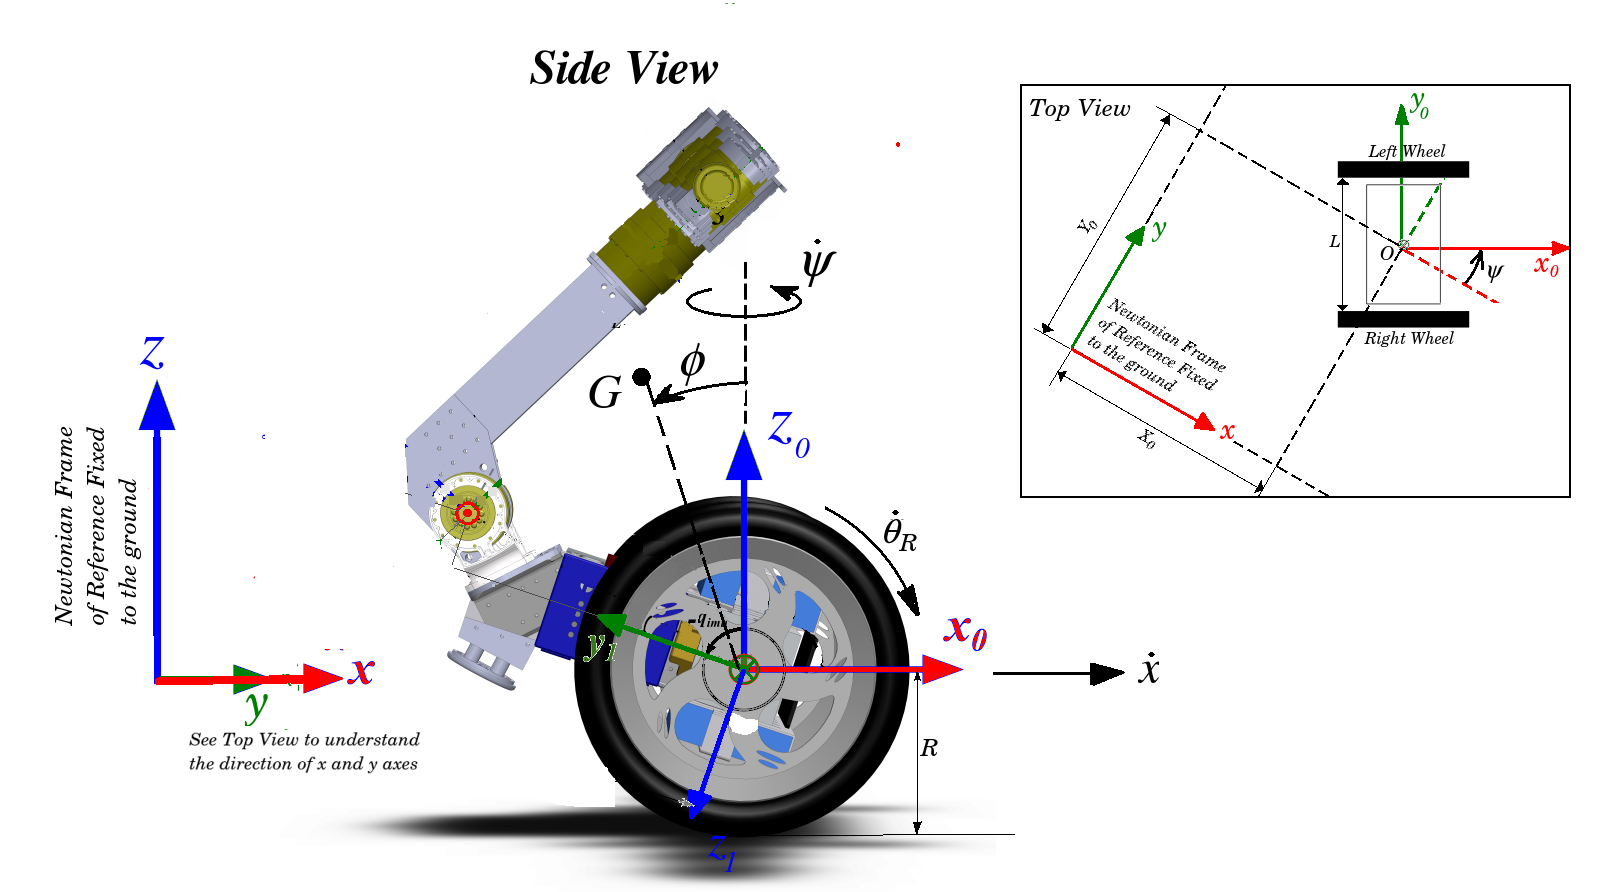
\includegraphics[width=\textwidth]{Figures/referenceImage.png}
 \caption{Frames of references on the robot}
 \label{fig:frames}
\end{figure}

Assumption: The pose of the body is fixed and only the wheels and the first link of the robot (i.e. the
base of Krang) are free to move.

Figure \ref{fig:frames} shows a simplified representation of side view the Krang robot. Define:

\begin{itemize}[label={}]
 \item[$O$] is the mid-point of the line connecting wheel-centers
 \item[$G$] is the center of gravity of the robot body
 \item[$\dot{x}$] is the heading speed of the robot
 \item[$\dot{\phi}$] is the rotation speed of $G$ about the wheel axis
 \item[$\dot{\psi}$] is the spin speed of the robot or the rate of change of heading direction
 \item[$L$] is the distance between wheel centers
 \item[$R$] is the radius of the wheel
 \item[$\tau_R, \tau_L$] is the torque applied by right and left wheel motors respectively 
 \item[$x_0y_0z_0$] is the frame of reference with origin at $O$, $x_0$ in the heading direction,
 $z_0$ always vertically upwards and $y_0$ pointing from right wheel to the left wheel
 \item[$x_1y_1z_1$] is the frame of reference fixed to the body with origin at $O$, $x_1$ opposite 
 to $y_0$ (from left to right wheel center), $y_1$ along the base of Krang (the first link above the wheels at angle $q_{imu}$ from
 $z_0$). When body pose is fixed $\dot{q}_{imu} = -\dot\phi$ i.e. $G$ rotates with the same speed as the base link. They increase/decrease
 in opposite direction though.
 \item[$m_B, m_w$] are the masses of robot body and one wheel respectively
 \item[$I_w$] $= \scalemath{0.75}{\left[\begin{matrix} \mathbf{XX}_w & 0 & 0 \\  
 0 & \mathbf{YY}_w & 0 \\ 
 0 & 0 & \mathbf{ZZ}_w \end{matrix}\right]}$
 \normalsize is the inertia matrix of the wheel wrt frame $x_0y_0z_0$
 \item[$\mathbf{MS}_B$] $=\left[\begin{matrix}\mathbf{MX}_B & \mathbf{MY}_B & \mathbf{MZ}_B\end{matrix}\right]^T$ is the mass times center of mass of the body expressed in frame $x_1y_1z_1$
 \item[$I_B$] $= \scalemath{0.75}{\left[\begin{matrix} \mathbf{XX}_B & \mathbf{XY}_B & \mathbf{XZ}_B \\
  \mathbf{XY}_B & \mathbf{YY}_B & \mathbf{YZ}_B \\ 
  \mathbf{XZ}_B & \mathbf{YZ}_B & \mathbf{ZZ}_B \end{matrix}\right]}$
  is the inertia matrix of the body wrt frame $x_1y_1z_1$ 
\end{itemize}

\section{Generalized Coordinates}

We select five generalized co-ordinates: $\{q\} = \{$ $X_0$, $Y_0$, $\theta_L$, $\theta_R$ and $\phi \}$. Where:
\begin{itemize}[label={}]
 \item[$X_0, Y_0$] are the position coordintes of $O$ wrt a Newtonian reference frame $xyz$ fixed on ground
 \item[$\theta_L, \theta_R$] are the rotation angles of the left and right wheels respectively
\end{itemize}

Given this Newtonian frame of reference we can define $\psi$ as the heading direction ($x_0$) measured as
an angle from the $x$-axis of the Newtonian frame.

\section{Constraint Equations}
Let $\bar{i}_0$, $\bar{j}_0$ and $\bar{k}_0$ be the unit vectors in frame $x_0y_0z_0$ and $\bar{I}$, $\bar{J}$ and 
$\bar{K}$ be the unit vectors in frame $xyz$.

Under the assumption of no slipping/skidding, we have two constraint equations:

\begin{align} 
 \bar{v}_L &= R\dot\theta_L\bar{i}_0 \label{constraintOne}\\
 \bar{v}_R &= R\dot\theta_R\bar{i}_0 \label{constraintTwo}
\end{align}

Since
\begin{align}
 \bar{v}_L &= \bar{v}_0 + \bar\omega_0 \times \bar{r}_{L/O} \nonumber \\
 &= \dot{X}_0 \bar{I} + \dot{Y}_0 \bar{J} + \dot{\psi} \bar{K} \times (\frac{L}{2}\bar{j}_0) \nonumber \\
 &= \dot{X}_0 (cos\psi\bar{i}_0 - sin\psi\bar{j}_0) + \dot{Y}_0 (sin\psi\bar{i}_0+cos\psi\bar{k}_0) - \frac{L}{2}\dot{\psi} \bar{i}_0 \nonumber \\
 &= (\dot{X}_0 cos\psi + \dot{Y}_0 sin\psi - \frac{L}{2}\dot{\psi}) \bar{i}_0 - (\dot{X}_0 sin\psi - \dot{Y}_0 cos\psi)\bar{j}_0 \nonumber 
\end{align}

And similarly,
\begin{align}
 \bar{v}_R  &= (\dot{X}_0 cos\psi + \dot{Y}_0 sin\psi + \frac{L}{2}\dot{\psi}) \bar{i}_0 - (\dot{X}_0 sin\psi - \dot{Y}_0 cos\psi)\bar{j}_0 \nonumber 
\end{align}

Comparing the coefficients of $\bar{i}_0$ in eqs. \ref{constraintOne}-\ref{constraintTwo} gives:
\begin{align}
 \dot{X}_0 cos\psi + \dot{Y}_0 sin\psi - \frac{L}{2}\dot{\psi} &= R\dot\theta_L \label{thetaL} \\
 \dot{X}_0 cos\psi + \dot{Y}_0 sin\psi + \frac{L}{2}\dot{\psi} &= R\dot\theta_R \label{thetaR} 
\end{align}
Subtraction and addition of the two equations gives us:
\begin{align}
 \dot{\psi} &= \frac{R}{L}(\dot\theta_R - \dot\theta_L) \label{psiThetaRelationship} \\
 \dot{X}_0 cos\psi + \dot{Y}_0 sin\psi &= \frac{R}{2}(\dot\theta_L + \dot\theta_R) \label{constraint1} 
\end{align}
Eq. \ref{psiThetaRelationship} can be integrated to give $\psi = \frac{R}{L}(\theta_R - \theta_L)$ which can be substituted in
eq. \ref{constraint1} to give our first constraint equation relating all generalized co-ordinates.

Comparing the coefficients of $\bar{j}_0$ in eqs. \ref{constraintOne}-\ref{constraintTwo} gives us our second constraint equation:
\begin{align}
 \dot{X}_0 sin\psi - \dot{Y}_0 cos\psi &= 0 \label{constraint2}
\end{align}

Eqs. \ref{constraint1}-\ref{constraint2} give the two equations relating our generalized velocities as a 
result of the nonholonomic constrainsts. Five generalized coordinates with two constraint equations leads
to three degrees of freedom.

\section{Defining Generalized Velocities}
It is easier to derive the dynamic model of the system in terms of the generalized velocities:
$\{\dot{q}\} = \{$ $\dot{x}$, $\dot{\phi}$, $\dot{\psi} \}$. These three velocities can take
arbitrary values all of whom will be kinematically admissible. In other words, they represent
our three degrees of freedom. Here $\dot{x}$ should be refered
to as a quasi-velocity as this velocity has meaning only as a veolocity but its corresponding
position variable $x$ does not give any physical meaning. Although, the infinitesimal change of
position $\delta x = \dot{x} dt$ (sometimes refered to as virtual displacement) has physical
meaning.

The older generalized velocities can be calculated from the new ones as follows:
\begin{align}
 \dot{X}_0 &= \dot{x}cos\psi \label{relStart}\\
 \dot{Y}_0 &= \dot{x}sin\psi \\
 \dot\theta_L &= \frac{1}{R}\dot{x} - \frac{L}{2R}\dot{\psi} \\
 \dot\theta_R &= \frac{1}{R}\dot{x} + \frac{L}{2R}\dot{\psi} \\
 \dot\phi &= \dot\phi \label{relEnd}
\end{align}
Where the first two relationships are derived by comparing the coefficients in 
$\dot{X}_0\bar{I}+\dot{Y}_0\bar{J} = \bar{v}_0 = \dot{x}\bar{i}_0 = \dot{x}(cos\psi\bar{I}+sin\psi\bar{J})$.
And the next
two relationships are derived by substituting the the first two relationships in eqs. \ref{thetaL}-\ref{thetaR}.
When these relationships (\ref{relStart}-\ref{relEnd}) are substituted in our constraint equations \ref{constraint1}-\ref{constraint2}, both
sides of the equations vanish. Indicating that these three degrees of freedom are not bound by any constraint.
We will now derive three dynamic equations in terms of our new generalized velocities. Those equations in
conjunction with these relationships can solve for all five generalized coordinates.

\section{Dynamic Equations}
Since we are dealing with quasi-velocities, we will use Kane's method to derive the dynamic equations. 

\subsection{Introduction to Kane's formulation}

The Kane's formulation is as follows:
\begin{align}
 \sum_{\substack{k}} \left[ m_k \bar{a}_{Gk} \cdot \left(\bar{v}_{Gk}\right)_j + \left( \frac{d\bar{H}_{Gk}}{dt} 
 \right) \cdot \left( \bar\omega_k \right)_j \right] = \sum_{\substack{n}}  \bar{F}_n \cdot \left( \bar{v}_n \right)_j 
 + \sum_{\substack{n}}  \bar{M}_m \cdot \left( \bar{\omega}_m \right)_j \;\; j=1 ... K \label{kanes}
\end{align}
where 
\begin{itemize}[label={}]
\item[$j$] is the unique number identifying each generalized co-ordinate in the system
\item[$k$] is the unique number identifying each rigid body in the system
\item[$n$] is the unique number identifying each external force acting on the system
\item[$m$] is the unique number identifying each external torque acting on the system
\item[$m_k$] is the mass of the $k$th body
\item[$\bar{a}_{Gk}$] is the acceleration of the center of mass of $k$th body
\item[$\bar{v}_{Gk}$] is the velocity of the center of mass of the $k$th body
\item[$\bar{H}_{Gk}$] is the angular momentum of body $k$ about its center of mass
\item[$\bar{\omega}_{k}$] is the angular velocity of the body $k$
\item[$F_n$] is the $n$th external force
\item[$M_m$] is the $m$th external moment
\item[$\bar{v}_{n}$] is the velocity of the point at which external Force $F_n$ is acting
\item[$\bar{\omega}_{m}$] is the angular velocity of the body on which torque is acting relative to the actuator applying the torque
\item[$()_j$] $=\frac{\partial ()}{\partial \dot{q}_j}$ the partial derivative of the quantity in brackets $()$ with respect to the generalized
velocity $\dot{q}_j$
\end{itemize}

\subsection{Kane's Left-Hand Side}
The left hand side of the Kane's equation containes a sum whose range is equal to the number of bodies
in the system. We have three bodies: Left-wheel ($L$), right wheel ($R$) and the body of robot ($B$). 
Each term in the sum consists of the acceleration ($\bar{a}_{Gk}$), velocity ($\bar{v}_{Gk}$), 
angular momentum ($\bar{H}_{Gk}$) of the center of mass and the body's angular velocity ($\bar{\omega}_k$). 
And then some partieal derivatives wrt to the generalized coordinates 
($(\bar{\omega}_k)_j=\frac{\partial \bar{\omega}_k}{\partial \dot{q}_j}$ and 
$(\bar{v}_{Gk})_j=\frac{\partial \bar{v}_{Gk}}{\partial \dot{q}_j}$). We will have three equations 
corresponding to each generalized coordinate $\{\dot{q}_j\} = \{$ $\dot{x}$, $\dot{\phi}$, $\dot{\psi} \}$.

\subsubsection{Left Wheel}
This evaluation takes place in the $x_Ly_Lz_L$ frame fixed to the left wheel such that it is parallel to 
frame $x_0y_0z_0$ when $\theta_L = 0$. So $\bar{i}_0 = cos\theta_L\bar{i}_L+sin\theta_L\bar{k}_L$, 
$\bar{j}_0 = \bar{j}_L$ and $\bar{k}_0 = -sin\theta_L\bar{i}_L+cos\theta_L\bar{k}_L$.
Angular velocity:
\begin{align}
 \bar{\omega}_L &= \dot\psi\bar{k}_0 + \dot\theta_L\bar{j_0} \nonumber \\
 &= \dot\psi\bar{k}_0 + \left(\frac{1}{R}\dot{x}-\frac{L}{2R}\dot\psi\right)\bar{j}_0 \nonumber \\
 &= -\dot\psi sin\theta_L\bar{i}_L + \left(\frac{1}{R}\dot{x}-\frac{L}{2R}\dot\psi\right)\bar{j}_L + \dot\psi cos\theta_L\bar{k}_L \label{kanesLHSVariableStart}
\end{align}
The terms that follow are also similarly to be expressed in frame $x_Ly_Lz_L$ but that step is skipped for brevity.
Velocity:
\begin{align}
  \bar{v}_{GL} &= \bar{v}_0 + \bar{\omega}_0 \times \bar{r}_{L/O} \nonumber \\
 &= \dot{x}\bar{i}_0 + \dot\psi\bar{k}_0 \times \frac{L}{2}\bar{j}_0 \nonumber \\
 &= \left(\dot{x}-\frac{L}{2}\dot\psi\right)\bar{i}_0  
\end{align}
Linear acceleration:
\begin{align}
 \bar{a}_{GL} &= \bar{a}_0 + \bar\alpha_0 \times \bar{r}_{L/O} + \bar\omega_0 \times \left( \omega_0 \times \bar{r}_{L/O}\right) \nonumber \\
 &= \ddot{x}\bar{i}_0 + \dot{x}\left(\dot\psi\bar{k}_0 \times \bar{i}_0\right)+ \ddot\psi\bar{k}_0 \times \frac{L}{2}\bar{j}_0 + \dot\psi\bar{k}_0 \times \left( \dot\psi\bar{k}_0 \times \frac{L}{2}\bar{j}_0\right) \nonumber \\
 &= \left(\ddot{x}-\frac{L}{2}\ddot\psi\right)\bar{i}_0 + \left(\dot{x}\dot\psi- \frac{L}{2}\dot\psi^2\right)\bar{j}_0  
\end{align}
Angular momentum and its derivative:
\begin{align}
 \bar{H}_{GL} &= I_w\bar{\omega}_L \nonumber \\
 \frac{d\bar{H}_{GL}}{dt} &= \frac{\partial \bar{H}_{GL}}{\partial t} + \bar\omega_L \times \bar{H}_{GL} \nonumber \\
\end{align}
where $I_w = \scalemath{0.75}{\left[\begin{matrix} \mathbf{ZZ}_w & 0 & 0 \\  0 & \mathbf{YY}_w & 0 \\ 0 & 0 & \mathbf{ZZ}_w \end{matrix}\right]}$. Due to symmetry the off-diogonal terms in the inertia matrix vanish, and the 
inertia about $x_L$-axis and $z_L$-axis are both equal (signified by $\mathbf{ZZ}_w$).

\subsubsection{Right Wheel}
This evaluation takes place in the $x_Ry_Rz_R$ frame fixed to the right wheel such that it is parallel to 
frame $x_0y_0z_0$ when $\theta_R = 0$. So $\bar{i}_0 = cos\theta_R\bar{i}_R+sin\theta_R\bar{k}_R$, 
$\bar{j}_0 = \bar{j}_R$ and $\bar{k}_0 = -sin\theta_R\bar{i}_R+cos\theta_R\bar{k}_R$.
Angular velocity:
\begin{align}
 \bar{\omega}_R &= \dot\psi\bar{k}_0 + \dot\theta_R\bar{j_0} \nonumber \\
 &= \dot\psi\bar{k}_0 + \left(\frac{1}{R}\dot{x}+\frac{L}{2R}\dot\psi\right)\bar{j}_0 \nonumber \\
 &= -\dot\psi sin\theta_L\bar{i}_R + \left(\frac{1}{R}\dot{x}+\frac{L}{2R}\dot\psi\right)\bar{j}_R + \dot\psi cos\theta_L\bar{k}_R 
\end{align}
The terms that follow are also similarly to be expressed in frame $x_Ry_Rz_R$ but that step is skipped for brevity.
Velocity:
\begin{align}
  \bar{v}_{GR} &= \bar{v}_0 + \bar{\omega}_0 \times \bar{r}_{R/O} \nonumber \\
 &= \dot{x}\bar{i}_0 + \dot\psi\bar{k}_0 \times \left(-\frac{L}{2}\bar{j}_0\right) \nonumber \\
 &= \left(\dot{x}+\frac{L}{2}\dot\psi\right)\bar{i}_0  
\end{align}
Linear acceleration:
\begin{align}
 \bar{a}_{GR} &= \bar{a}_0 + \bar\alpha_0 \times \bar{r}_{R/O} + \bar\omega_0 \times \left( \omega_0 \times \bar{r}_{R/O}\right) \nonumber \\
 &= \ddot{x}\bar{i}_0 + \dot{x}\left(\dot\psi\bar{k}_0 \times \bar{i}_0\right)+ \ddot\psi\bar{k}_0 \times \left(-\frac{L}{2}\bar{j}_0\right) + \dot\psi\bar{k}_0 \times \left( \dot\psi\bar{k}_0 \times \left(-\frac{L}{2}\bar{j}_0\right)\right) \nonumber \\
 &= \left(\ddot{x}+\frac{L}{2}\ddot\psi\right)\bar{i}_0 + \left(\dot{x}\dot\psi + \frac{L}{2}\dot\psi^2\right)\bar{j}_0  
\end{align}
Angular momentum and its derivative:
\begin{align}
 \bar{H}_{GR} &= I_w\bar{\omega}_R \nonumber \\
 \frac{d\bar{H}_{GR}}{dt} &= \frac{\partial \bar{H}_{GR}}{\partial t} + \bar\omega_0 \times \bar{H}_{GR} \nonumber \\
\end{align}

\subsubsection{Body}
We will evaluate the quantities in frame $x_1y_1z_1$. It is useful to know that $\bar{i}_0=sinq_{imu}\bar{j}_1-cosq_{imu}\bar{k}_1$,
$\bar{j}_0=-\bar{i}_1$ and $\bar{k}_0=cosq_{imu}\bar{j}_1+sinq_{imu}\bar{k}_1$,
For brevity we will leave the expressions in closed forms.\\
Angular velocity:
\begin{align}
 \bar{\omega}_B &= \dot\psi\bar{k}_0 + \dot\phi\bar{i}_1 
\end{align}
Expressing $\bar{k}_0$ in frame $x_1y_1z_1$ gives us the expression in this frame.
\\Velocity:
\begin{align}
  \bar{v}_{GB} &= \bar{v}_0 + \bar{\omega}_B \times \bar{r}_{B/O} \nonumber \\
  &= \dot{x}\bar{i}_0 + \bar{\omega}_B \times \frac{1}{m_B}\mathbf{MS}_{B} 
\end{align}isa
Linear acceleration:
\begin{align}
 \bar{a}_{GB} &= \bar{a}_0 + \bar\alpha_B \times \bar{r}_{B/O} + \bar\omega_B \times \left( \omega_B \times \bar{r}_{B/O}\right) 
\end{align}
where 
\begin{align} \begin{split}
 &\bar{a}_0 = \frac{d\bar{v}_0}{dt} = \frac{d\left(\dot{x}\bar{i}_0\right)}{dt} 
 = \ddot{x}\bar{i}_0+\dot{x}\left(\dot\psi\bar{k}_0 \times \bar{i}_0\right)  \\
 &\bar\alpha_B = \frac{d\bar{\omega}_B}{dt} = \frac{d\left(\dot\psi\bar{k}_0 + \dot\phi\bar{i}_1 \right)}{dt}
 = \ddot\psi\bar{k}_0 + \ddot\phi\bar{i}_1 + \dot\phi\left(\bar\omega_B \times \bar{i}_1\right) \label{a0alphaB}
\end{split} \end{align}
Angular momentum and its derivative:
\begin{align}
 \bar{H}_{GB} &= I_B\bar{\omega}_B \nonumber \\
 \frac{d\bar{H}_{GB}}{dt} &= \frac{\partial \bar{H}_{GB}}{\partial t} + \bar\omega_B \times \bar{H}_{GB} \label{kanesLHSVariableEnd}
\end{align}

\subsubsection{Left-Hand Side Final Evaluation}
The Kanes' formulation (Eq. \ref{kanes}) are in fact three equation each corresponding to a different generalized velocity
${\dot{q}_j} = {\dot{x},\dot\psi,\dot\phi}$. Each of these three equation is a summation of the given expression evaluated
for each body ${k}={L,R,B}$ i.e. Left-wheel, right-wheel and body. When the expressions that we evaluated in eqs. 
\ref{kanesLHSVariableStart}-\ref{kanesLHSVariableEnd} are substituted in Kanes' equations (Eq. \ref{kanes}) and the results 
evaluted (using MATLAB code listed in the Appendix section \ref{app1}), we get the following expression:
\begin{align}
 &\mathbf{A\ddot{q}+C\dot{q}} \nonumber
\end{align}\\
where
\begin{align} \begin{split}
 &\mathbf{A}=\scalemath{0.75}{\left[\begin{matrix}
  m_B+2m_w+\frac{2\mathbf{YY}_w}{R^2} &
  \mathbf{MX}_b &
  -\mathbb{M}_1 \\
  \mathbf{MX}_b &
  \frac{m_wL^2}{2}+\frac{\mathbf{YY}_wL^2}{2R^2}+2\mathbf{ZZ}_w+\frac{\mathbb{M}_2^2}{m_b}+\mathbb{M}_3 + \frac{\mathbf{MX}_b^2}{m_B} &
  \mathbb{M}_4 \\
  -\mathbb{M}_1 &
  \mathbb{M}_4 &
  \mathbb{M}_6+\mathbf{XX}_b
  \end{matrix}\right]}  \\
 &\mathbf{C}=\scalemath{0.75}{\left[\begin{matrix}
  0 &
  \mathbb{M}_2\dot\psi &
  \mathbb{M}_2\dot\phi \\
  -\frac{1}{2}\mathbb{M}_2\dot\psi &  
  -\frac{1}{2}\mathbb{M}_2\dot{x}+\frac{1}{2}\mathbb{M}_7\dot\phi &
  \mathbb{M}_5\dot\phi+\frac{1}{2}\mathbb{M}_7\dot\psi \\
  0 &
  \mathbb{M}_8-\frac{1}{m_b}\mathbb{M}_1\mathbb{M}_2 &
  0
 \end{matrix}\right]} \label{kanesAC}
\end{split}\end{align}\\
where
\begin{align}
 \mathbb{M}_1 &= \left(\mathbf{MY}_bcosq_{imu}+\mathbf{MZ}_bsinq_{imu}\right) \nonumber \\
 \mathbb{M}_2 &= \mathbf{MZ}_bcosq_{imu}-\mathbf{MY}_bsinq_{imu} \nonumber \\
 \mathbb{M}_3 &= \mathbf{ZZ}_bsin^2q_{imu}+\mathbf{YY}_bcos^2q_{imu}+\mathbf{YZ}_bcosq_{imu}sinq_{imu} \nonumber \\
 \mathbb{M}_4 &= \mathbf{XZ}_bsinq_{imu}+\mathbf{XY}_bcosq_{imu}+\frac{\mathbf{MX}_b}{m_B}\mathbb{M}_1 \nonumber \\
 \mathbb{M}_5 &= -\mathbf{XZ}_bcosq_{imu}+\mathbf{XY}_bsinq_{imu}+\frac{\mathbf{MX}_b}{m_B}\mathbb{M}_2 \nonumber \\
 \mathbb{M}_6 &= \frac{1}{m_B}\left(\mathbf{MY}_b^2+\mathbf{MZ}_b^2\right) \nonumber \\
 \mathbb{M}_7 &= \frac{1}{m_B}\left(\left(\mathbf{MZ}_b^2-\mathbf{MY}_b^2\right)sin2q_{imu}+2\mathbf{MX}_b\mathbf{MZ}_bcos2q_{imu}\right) - 2\mathbb{M}_8 \nonumber \\
 \mathbb{M}_8 &= \mathbf{YZ}_bcos2q_{imu}+\left(\mathbf{ZZ}_b-\mathbf{YY}_b\right)cosq_{imu}sinq_{imu} \nonumber 
\end{align}
The matrices $\mathbf{A}$ amd $\mathbf{C}$ are saved in the symbolic variables \texttt{AA} and \texttt{CC} generated by the code.

\subsubsection{Comparing with \cite{kim2005dynamic}}

\bf{Deriving Expressions in \cite{kim2005dynamic}}
\normalfont\\
A similar dynamic model has been derived by \cite{kim2005dynamic}. From the closed form expressions of their paper they
have directly stated thier final expressions while skipping the details of derivations. In order to ascertain
the correctness of their work, we derive the expressions on our own by substituting the velocities, accelerations etc
they derived in the closed form expressions. This is done using MATLAB code listed in appendix (section \ref{app2}).
These are the resulting expressions for the left-hand sides of the threee equations:
\begin{align}
 F_1 &= \scalemath{0.8}{-\frac{1}{R^2}(2R^2\ddot{x}m_C + 2I_{w3}\ddot{x} + R^2\ddot{x}m_S - R^2d\ddot{\phi}m_Scos\phi + R^2d\dot{\phi}^2m_Ssin\phi + R^2d\dot{\psi}^2m_Ssin\phi)} \nonumber \\
     &= \scalemath{0.8}{-2\ddot{x}m_C - \frac{2I_{w3}}{R^2}\ddot{x} - \ddot{x}m_S + d\ddot{\phi}m_Scos\phi - d\dot{\phi}^2m_Ssin\phi - d\dot{\psi}^2m_Ssin\phi} \nonumber \\
     &= \scalemath{0.8}{-(m_S + 2m_C + \frac{2I_{w3}}{R^2})\ddot{x} + m_Sdcos\phi\ddot{\phi} - m_Sdsin\phi(\dot{\phi}^2 + \dot{\psi}^2)} \nonumber \\
 F_2 &= \scalemath{0.8}{-\frac{1}{R^2}(2I_{w3}L^2\ddot{\psi} + I_2R^2\ddot{\psi} + 2I_{w2}R^2\ddot{\psi} + 2L^2R^2\ddot{\psi}m_C + R^2d^2\ddot{\psi}m_Ssin\phi^2} \nonumber \\ 
         & \hskip 3em + \scalemath{0.8}{\frac{1}{2}R^2d^2\dot{\phi}\dot{\psi}m_Ssin(2\phi))} \nonumber \\
     &= \scalemath{0.8}{-\frac{2I_{w3}L^2}{R^2}\ddot{\psi} - I_2\ddot{\psi} - 2I_{w2}\ddot{\psi} - 2L^2\ddot{\psi}m_C - d^2\ddot{\psi}m_Ssin\phi^2 - \frac{1}{2}d^2\dot{\phi}\dot{\psi}m_Ssin(2\phi)} \nonumber \\
     &= \scalemath{0.8}{-(2m_CL^2 +\frac{2I_{w3}L^2}{R^2} + 2I_{w2} + m_Sd^2sin\phi^2 + I_2 )\ddot{\psi} - m_Sd^2sin\phi cos\phi\dot{\phi}\dot{\psi}} \nonumber \\
 F_3 &= \scalemath{0.8}{-d^2\ddot{\phi}m_S - I_3\ddot{\phi} + d\ddot{x}m_Scos\phi + \frac{1}{2}(d^2\dot{\psi}^2m_Ssin(2\phi))} \nonumber \\
     &= \scalemath{0.8}{-(m_Sd^2 + I_3)\ddot{\phi} + m_Sdcos\phi\ddot{x} + m_Sd^2sin\phi cos\phi\dot{\psi}^2} \nonumber  
\end{align}
The expressions match exactly as are there in the paper if $I_{w3} = \frac{m_CR^2}{2}$ and $I_{w2} = \frac{m_C}{4R^2}$.
The paper has made a typo in the last equation using $\dot{\phi}^2$ instead of $\dot{\psi}^2$. 

We can write down the $A$ and $C$ matrices using the above equations so that it becomes easier to match it 
term by term with our derived equations. So we have:

\begin{align} \begin{split}
 &\mathbf{A} = \scalemath{0.75}{\left[ \begin{matrix} -(m_S + 2m_C + \frac{2I_{w3}}{R^2}) & 0 & m_Sdcos\phi \\ 
   0 & -(2m_CL^2 +\frac{2I_{w3}L^2}{R^2} + 2I_{w2} + m_Sd^2sin\phi^2 + I_2 ) & 0 \\
   m_Sdcos\phi & 0  & -(m_Sd^2 + I_3) \end{matrix} \right]} \\
 &\mathbf{C} = \scalemath{0.75}{\left[ \begin{matrix} 0 & - m_Sdsin\phi\dot{\psi} & - m_Sdsin\phi\dot{\phi} \\ 
     0 & - m_Sd^2sin\phi cos\phi\dot{\phi} & 0 \\ 
    0 & m_Sd^2sin\phi cos\phi\dot{\psi} & 0 \end{matrix} \right]} \label{kimAC}
\end{split} \end{align}
\\
\bf{Substituting \cite{kim2005dynamic}'s assumptions, symbols and equivalent expressions in place of ours}
\normalfont\\
In order to compare our work with \cite{kim2005dynamic} we re-write our derived expression in terms of the
symbols used by \cite{kim2005dynamic}. In this subsection we will write down definitions of symbols used by
us in terms of equivalent expressions consisting of the symbols used by \cite{kim2005dynamic}. 

The symbols they used for the masses of the body and the wheel are $m_S$ and $m_C$ respectively. The distance between wheel centers
they assumed is $2L$. So:
\begin{align}
 m_B = m_S \hspace{35pt} m_w = m_C \hspace{35pt} L=2L \label{subsStart}
\end{align}
\\
The inertia terms for the wheel are as follows:
\begin{align}
 I_w &= \scalemath{0.75}{\left[\begin{matrix} \mathbf{XX}_w & 0 & 0 \\  
 0 & \mathbf{YY}_w & 0 \\ 
 0 & 0 & \mathbf{ZZ}_w \end{matrix}\right]}
 = \scalemath{0.75}{\left[\begin{matrix} I_{w2} & 0 & 0 \\  
 0 & I_{w3} & 0 \\ 
 0 & 0 & I_{w2} \end{matrix}\right]}
\end{align}
\\
The radial distance from 
$O$ to center of mass $G$ is assumed in the paper to be $d$. This means our mass times COM parameter becomes:
\begin{align}
 \mathbf{MS}_b &= \left[\begin{matrix} \mathbf{MX}_b & \mathbf{MY}_b & \mathbf{MZ}_b \end{matrix}\right]^T = \left[\begin{matrix} 0 & m_Sdcos\kappa & m_Sdsin\kappa \end{matrix}\right]^T  
\end{align} \\ where $\kappa = q_{imu} + \phi$ is the angle from $y_1$-axis to $\overline{OG}$ (see Fig. \ref{fig:kimAnglesInertias}A).
\begin{figure}[ht]
 \centering
 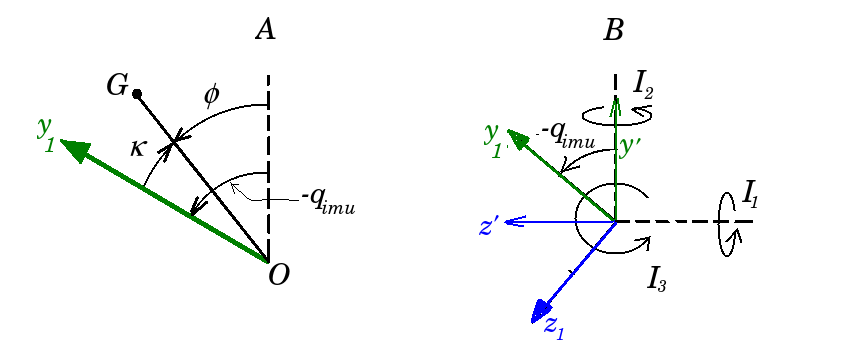
\includegraphics[width=\textwidth]{Figures/angles.png}
 \caption{A. Understanding the definition of angles in our analysis. Follow the arrows and you get: $-q_{imu}+\kappa=\phi$ or $\kappa=q_{imu}+\phi$
 \hspace{20pt}B. Inertias as defined in \cite{kim2005dynamic}}
 \label{fig:kimAnglesInertias}
\end{figure}

Finally the inertia for body in \cite{kim2005dynamic} is assumed to be $I_3$ about the wheel-axis, $I_2$ about the fixed vertical
and $I_1$ about the forward direction (see Fig. \ref{fig:kimAnglesInertias}B). In order to find the equivalent expressions for the
inertia parameters of the body we defined for our analysis we will have to perform rotation transformation of the inertia
as defined in \cite{kim2005dynamic} to express it in the frame we defined in our analysis i.e. frame $x_1y_1z_1$. The formula for rotation transformation
is:
\[
 I'=R\;I\;R^T
\]
\\where $I$ is the inertia matrix with respect to (say) frame 1 and $I'$ is the same in frame 2
and $R$ is the rotation transformation that transforms a vector $\omega$ expressed in frame 1 to $\omega'$
in frame 2.
\[
 \omega' = R\;\omega
\]
In our case we have an inertia matrix $\scalemath{0.75}{\left[\begin{matrix} I_3 & 0 & 0 \\ 0 & I_2 & 0 \\ 0 & 0 & I_1 \end{matrix}\right]}$ defined in
frame $x'y'z'$ (see Fig. \ref{fig:kimAnglesInertias}B) and we need to rotate it into frame $x_1y_1z_1$. The rotation transformation
will be:
\[
 R=\scalemath{0.75}{\left[\begin{matrix} 1 & 0 & 0 \\ 0 & cosq_{imu} & -sinq_{imu} \\ 0 & sinq_{imu} & cosq_{imu} \end{matrix}\right]}
\]
\\Applying these concepts we find that:
\begin{align}
 \scalemath{0.75}{\left[\begin{matrix} \mathbf{XX}_B & \mathbf{XY}_B & \mathbf{XZ}_B \\
  \mathbf{XY}_B & \mathbf{YY}_B & \mathbf{YZ}_B \\ 
  \mathbf{XZ}_B & \mathbf{YZ}_B & \mathbf{ZZ}_B \end{matrix}\right]} &=
  \scalemath{0.75}{\left[\begin{matrix} I_3 & 0 & 0 \\ 
   0 & I_1sin^2q_{imu}+I_2cos^2q_{imu} & \left(I_2-I_1\right)cosq_{imu}sinq_{imu} \\ 
   0 & \left(I_2-I_1\right)cosq_{imu}sinq_{imu} & I_1cos^2q_{imu}+I_2sin^2q_{imu} \end{matrix}\right]} \label{subsEnd}
\end{align}\\
\bf{Result of Substitution}
\normalfont\\
Applying the substitutions described in eqs. \ref{subsStart}-\ref{subsEnd} on the matrices 
$\mathbf{A}$ and $\mathbf{C}$ (eq. \ref{kanesAC}), we get the following results. These results
are evaluated in the MATLAB code (section \ref{app1}) and saved in symbolic vairables \texttt{Acheck}
and \texttt{Ccheck}.
\begin{align} \begin{split}
 &\mathbf{A} = \scalemath{0.75}{\left[ \begin{matrix} m_S + 2m_C + \frac{2I_{w3}}{R^2} & 0 & -m_Sdcos\phi \\ 
   0 & 2m_CL^2 +\frac{2I_{w3}L^2}{R^2} + 2I_{w2} + m_Sd^2sin\phi^2 + I_2  & 0 \\
   -m_Sdcos\phi & 0  & m_Sd^2 + I_3 \end{matrix} \right]} \\
 &\mathbf{C} = \scalemath{0.75}{\left[ \begin{matrix} 0 & m_Sdsin\phi\dot{\psi} & m_Sdsin\phi\dot{\phi} \\ 
    -\frac{1}{2}m_Sdsin\phi\dot\psi & -\frac{1}{2}m_Sdsin\phi\dot{x}+\frac{1}{2}m_Sd^2sin2\phi\dot{\phi} & \frac{1}{2}m_Sd^2sin2\phi\dot{\psi} \\ 
    0 & -\frac{1}{2}m_Sd^2sin2\phi\dot{\psi} & 0 \end{matrix} \right]} \label{subsResult}
\end{split} \end{align}
Comparing with the matrices derived in \cite{kim2005dynamic} shown in eq. \ref{kimAC} we see that all the terms are 
identical except that the signs of all terms are opposite which only indicates that the expressions evaluated
from \cite{kim2005dynamic} are on the other side of the equation. One other exception is in row 2 of the 
$\mathbf{C}$ matrix where we see some additional terms in our analysis that are not present in \cite{kim2005dynamic}. 
To understand the differences, let's looks at the final expression, which we can find by multiplying $\mathbf{C}$ with $\mathbf{\dot{q}}$ 
and look at the form of the second element of the resulting vector.
For \cite{kim2005dynamic}, we get:
\[
 \left[\mathbf{C\dot{q}}\right]_2 = -m_Sd^2sin\phi cos\phi\dot\phi\dot\psi
\]
For our analysis, we get:
\begin{align}
 \left[\mathbf{C\dot{q}}\right]_2 &= -\frac{1}{2}m_Sdsin\phi\dot\psi\dot{x} -\frac{1}{2}m_Sdsin\phi\dot{x}\dot\psi+\frac{1}{2}m_Sd^2sin2\phi\dot{\phi}\dot\psi + \frac{1}{2}m_Sd^2sin2\phi\dot{\psi}\dot\phi \nonumber \\
 &= -m_Sdsin\phi\dot\psi\dot{x} + m_Sd^2sin2\phi\dot{\phi}\dot\psi \nonumber \\
 &= -m_Sdsin\phi\dot\psi\dot{x} + 2m_Sd^2sin\phi cos\phi\dot{\phi}\dot\psi \nonumber
\end{align}
So there is an additional $-m_Sdsin\phi\dot\psi\dot{x}$ and there is a coefficient $2$ with the matching term $m_Sd^2sin\phi cos\phi\dot{\phi}\dot\psi$
that was not present in the expression from \cite{kim2005dynamic}. 

Both these differences are explained by pointing out errors in the derivation
of \cite{kim2005dynamic}. They did not evaluate the linear and angular acceleration of the body correctly. They forgot to take the derivative
of the unit vector when they evaluated $\frac{d{}^F\mathbf{v}^{S_C}}{dt}$ (\cite[eq.~10]{kim2005dynamic}) and ${}^F\alpha^S$(\cite[eq.~9]{kim2005dynamic}).
These terms are labeled as $\bar{a}_0$ and $\bar\alpha_B$ in our analysis and evaluated in eq.\ref{a0alphaB}. The reason why derivative of the
unit vectors is important is because these unit vectors are not fixed. When the body rotates the unit vectors $\bar{i}_0$ and $\bar{i}_1$ rotate
with angular speed $\dot\psi\bar{k}_0$. Using the symbols of \cite{kim2005dynamic} we will say unit vectors $\mathbf{n}_1$ and $\mathbf{n}_3$
rotate with a speed of $\dot\psi\mathbf{n}_2$ or $u_2\mathbf{n}_2$. This would mean that the correct evaluation of the two terms in \cite{kim2005dynamic} is as follows:
\begin{align}
 \frac{d{}^F\mathbf{v}^{S_C}}{dt} &= \frac{d\left(u_1\mathbf{n}_1\right)}{dt} = \dot{u}_1\mathbf{n}_1 + u_1\left(u_2\mathbf{n}_2 \times \mathbf{n}_1\right) \nonumber \\
  &= \dot{u}_1\mathbf{n}_1 - u_1u_2\mathbf{n}_3 \nonumber \\
 {}^F\alpha^S &= \frac{d\left({}^F\omega^S\right)}{dt} = \frac{d\left(u_2\mathbf{n}_2+u_3\mathbf{n}_3\right)}{dt}
 = \dot{u}_2\mathbf{n}_2+\dot{u}_3\mathbf{n}_3+u_3\left(u_2\mathbf{n}_2 \times \mathbf{n}_3\right) \nonumber \\
 &= \dot{u}_2\mathbf{n}_2+\dot{u}_3\mathbf{n}_3+u_2u_3\mathbf{n}_1 \nonumber 
\end{align}
When these new expressions are used for the evaluation of body's linear acceleration ${}^F\mathbf{a}^{S^*}$ 
(\cite[eq.~10]{kim2005dynamic}), we get:
\begin{align}
 {}^F\mathbf{a}^{S^*} &= \frac{d{}^F\mathbf{v}^{S_C}}{dt} + {}^F\alpha^S \times \overline{S^CS^*} + {}^F\omega^S \times \left( {}^F\omega^S \times \overline{S^CS^*} \right) \nonumber \\
 &= \scalemath{0.75}{
 \left[\begin{matrix} \dot{u}_1 \\ 0 \\ -u_1u_2 \end{matrix}\right]
 +\left[\begin{matrix} u_2u_3 \\ \dot{u}_2 \\ \dot{u}_3 \end{matrix}\right] \times \left[\begin{matrix} -dsin\phi \\ dcos\phi \\ 0 \end{matrix}\right]
 +\left[\begin{matrix} 0 \\ u_2 \\ u_3 \end{matrix}\right] \times \left(\left[\begin{matrix} 0 \\ u_2 \\ u_3 \end{matrix}\right] \times \left[\begin{matrix} -dsin\phi \\ dcos\phi \\ 0 \end{matrix}\right] \right)
 }\nonumber \\
 &= \scalemath{0.75}{\begin{matrix} 
  \left( \dot{u}_1 - \dot{u}_3dcos\phi +  (u_2^2 + u_3^2)dsin\phi \right)  \\
  +\left( -\dot{u}_3dsin\phi - u_3^2dcos\phi   \right)  \\
  +\left(\dot{u}_2dsin\phi + 2u_2u_3dcos\phi - u_1u_2   \right) 
 \end{matrix}
 \begin{matrix} \mathbf{n}_1 \\ \mathbf{n}_2 \\ \mathbf{n}_3 \end{matrix}} \label{correctedAcc}
\end{align}
This expressions matches the one derived in \cite[eq.~10]{kim2005dynamic} except that the last component has an additional 
$- u_1u_2$ and coefficient $2$ for the terms $u_2u_3dcos\phi$. Implementing these changes gives us the dynamic equations that match
exactly with the matrices that resulted from substitution at the beginning of this section (eq.\ref{subsResult}). This is implemented in the MATLAB code
in the appendix section \ref{app3}.

\subsection{Kane's Right Hand Side}

The right hand side of the Kane's forumulation \ref{kanes} is the sum of some dot product terms. Each term is either the
dot product of:
\begin{itemize}
 \item force applied on the system $\bar{F}_n$
 \item the linear velocity $\bar{v}_n$ of the point differentiated partially wrt the the unique gerneralized speed 
 $\dot{q}_j$ corresponding to each equation i.e. $\frac{\partial \bar{v}_n}{\partial \dot{q}_j}$\\
\end{itemize}
or the dot product of:
\begin{itemize}
 \item torque applied on the system $\bar{\tau}_n$
 \item the angular velocity $\bar{\omega}_n$ of the body differentiated partially wrt the the unique gerneralized speed 
 $\dot{q}_j$ corresponding to each equation i.e. $\frac{\partial \bar{\omega}_n}{\partial \dot{q}_j}$
\end{itemize}

So, in order to analyse the right-hand side of the equation, we need to list down all the forces and torques applied
to the system and the points at which they are being applied. They are as follows:
\begin{itemize}[label={}]
 \item[$\bar\tau_L, \bar\tau_R $] Torques applied by wheel motors (in the body) on the right wheel and left wheel at points 
 $R$ and $L$ on the wheels
 \item[$-\bar\tau_L, -\bar\tau_R $] Reaction torques applied on body at points $R$ and $L$ on the body
 \item[$\bar{F}_g$] $=m_Bg$ the weight of the body applied at point $G$
 \item[$\bar{F}_{el}, \bar{\tau}_{el}$] Force and torque applied by the environment on the left hand end-effector at point $E_l$
 \item[$\bar{F}_{er}, \bar{\tau}_{er}$] Force and torque applied by the environment on the right hand end-effector at point $E_r$
\end{itemize}

So there are nine forces/torques so far. Three can be further added to the list by analysing the forces $\bar{F}_g$, $\bar{F}_{el}$ and $\bar{F}_{er}$
wrt point $O$ so each of them is broken into a force-torque couple acting at point $O$. So:

\begin{itemize}[label={}]
 \item[$\bar{F}_g$] at $G$ gives the effect of force $\bar{F}_g$ and a torque $\bar{r}_{G/O} \times \bar{F}_g$ wrt $O$
 \item[$\bar{F}_{el}$] at $E_l$ gives the effect of force $\bar{F}_{el}$ and a torque $\bar{r}_{E_l/O} \times \bar{F}_{el}$ wrt $O$
 \item[$\bar{F}_{er}$] at $E_r$ gives the effect of force $\bar{F}_{er}$ and a torque $\bar{r}_{E_r/O} \times \bar{F}_{er}$ wrt $O$
\end{itemize}

Let $\scalemath{0.75}{\bar{F}_{el} = \left[\begin{matrix} F_{lx} & F_{ly} & F_{lz} \end{matrix}\right]^T}$, 
$\scalemath{0.75}{\bar{F}_{er} = \left[\begin{matrix} F_{rx} & F_{ry} & F_{rz} \end{matrix}\right]^T}$,
$\scalemath{0.75}{\bar{\tau}_{el} = \left[\begin{matrix} \tau_{lx} & \tau_{ly} & \tau_{lz} \end{matrix}\right]^T}$ and
$\scalemath{0.75}{\bar{\tau}_{er} = \left[\begin{matrix} \tau_{rx} & \tau_{ry} & \tau_{rz} \end{matrix}\right]^T}$ 
be the components of forces/torques defined in the frame $x_0y_0z_0$. Also
$\scalemath{0.75}{\bar{r}_{E_l/O} = \left[\begin{matrix} r_{lx} & r_{ly} & r_{lz} \end{matrix}\right]^T}$ and
$\scalemath{0.75}{\bar{r}_{E_r/O} = \left[\begin{matrix} r_{rx} & r_{ry} & r_{rz} \end{matrix}\right]^T}$ be the
position coordinates of the end effectors again presented in the frame $x_0y_0z_0$. Also 
$\scalemath{0.75}{\bar{F}_{g} = \left[\begin{matrix} 0 & 0 & -g \end{matrix}\right]^T}$.
Also $\bar{r}_{G/O}$ is to be expressed in the $x_0y_0z_0$ which will be
$\scalemath{0.75}{\bar{r}_{G/O} = \frac{1}{m_B}\left[\begin{matrix} 0 & sq_{imu} & -cq_{imu} \\ -1 & 0 & 0 \\ 0 & cq_{imu} & sq_{imu} \end{matrix}\right]
\left[\begin{matrix} \mathbf{MX}_{B} \\ \mathbf{MY}_{B} \\ \mathbf{MZ}_{B} \end{matrix}\right]}$.

\vspace{5mm}

We now give closed form expressions of terms contributed on the RHS by these forces and torques:

\vspace{5mm} 
\begin{enumerate}
 \item Forces at point $O$ will contribute the following terms:
\begin{align}
 &\left( \bar{F}_{er} + \bar{F}_{el} + \bar{F}_g  \right) \cdot \frac{\partial \bar{v}_0}{\partial \dot{q}_j}
\end{align}
where $\scalemath{0.75}{\bar{v}_{0} = \left[\begin{matrix} \dot{x} & 0 & 0 \end{matrix}\right]^T}$

\vspace{5mm}

 \item Torques at point $O$ will contribute the following terms:
\begin{align}
  &\left(\bar{r}_{G/O} \times \bar{F}_g + \bar{r}_{E_l/O} \times \bar{F}_{el} + \bar{r}_{E_r/O} \times \bar{F}_{er} 
  - \left(\bar\tau_L + \bar\tau_R\right)\bar{j}_0 + \bar\tau_{er} + \bar\tau_{el}\right) \cdot \frac{\partial \bar{\omega}_B}{\partial \dot{q}_j}
\end{align}
where $\bar{\omega}_B = - \dot\phi\bar{j}_0 + \dot\psi\bar{k}_0$

\vspace{5mm}

 \item Torque on the wheel at $L$ will contribute the following terms
\begin{align}
 & \tau_L\bar{j}_0  \frac{\partial \bar{\omega}_L}{\partial \dot{q}_j}
\end{align}
where $\bar{\omega}_L = \dot\psi\bar{k}_0 + \left(\frac{1}{R}\dot{x}-\frac{L}{2R}\dot\psi\right)\bar{j}_0$

\vspace{5mm}

 \item Torque on the wheel at $R$ will contribute the following terms
\begin{align}
 & \tau_R\bar{j}_0 \cdot \frac{\partial \bar{\omega}_R}{\partial \dot{q}_j}
\end{align}
where $\bar{\omega}_R = \dot\psi\bar{k}_0 + \left(\frac{1}{R}\dot{x}+\frac{L}{2R}\dot\psi\right)\bar{j}_0$
\end{enumerate}

The MATLAB script \texttt{kanesRHS.m} is used to evaluate the above closed-form expressions to give the final terms.
Vectors \texttt{a}, \texttt{b}, \texttt{c} and \texttt{d} store the three terms produced by each of the four closed form expressions listed
above. The result of the evaluation fives the following right hand sides:
\begin{itemize}[label={}]
 \item{eq1:} $\frac{\tau_L}{R} + \frac{\tau_R}{R} + F_{lx} + F_{rx}$
 \item{eq2:} $-\frac{L}{2R}\tau_L + \frac{L}{2R}\tau_R + \tau_{lz} + \tau_{rz} + r_{lx}F_{ly} - r_{ly}F_{lx} + r_{rx}F_{ry} - E_{ry}F_{rx}$
 \item{eq3:} $\tau_L + \tau_R + g\left(\mathbf{MZ}_Bcosq_imu - \mathbf{MY}_Bsinq_{imu}\right) - \tau_{ry} - \tau_{ly} + r_{lx}F_lz - r_{lz}F_{lx} + r_{rx}F_{rz} - r_{rz}F_{rx}$
\end{itemize}

\appendix

\section{MATLAB code for Evaluation of Kane's Equaiton}

\subsection{Kane's LHS} \label{app1}

This is the code listing for the evaluation of Kane's equation LHS (Eq. \ref{kanes}) for our robot:

\lstinputlisting[language=Matlab]{../../3-matlab/kanesWIPFinalized.m}


\subsection{Evaluation of Expressions in \cite{kim2005dynamic}} \label{app2}

This code is used to derive the final expressions from the closed form expressions in \cite{kim2005dynamic}.

\lstinputlisting[language=Matlab]{../../3-matlab/kim/dynamics.m}

\subsection{Evaluation of Expressions in \cite{kim2005dynamic} with Corrections} \label{app3}

This code is used to derive the final expressions from the closed form expressions in \cite{kim2005dynamic} with
corrected expression for ${}^F\mathbf{a}^{S^*}$ as mentioned in eq. \ref{correctedAcc}.

\lstinputlisting[language=Matlab]{../../3-matlab/kim/dynamicsCorrected.m}


\subsection{Kane's RHS} \label{app4}

This is the code listing for the evaluation of Kane's equation RHS (Eq. \ref{kanes}) for our robot:

\lstinputlisting[language=Matlab]{../../3-matlab/kanesRHS.m}


\bibliographystyle{plain}
\bibliography{reference}

\end{document}